\documentclass[10pt,a4paper]{article}
\usepackage[utf8]{inputenc}
\usepackage{amsmath}
\usepackage{amsfonts}
\usepackage{amssymb}
\usepackage{graphicx}
\usepackage{gensymb}
\title{The Riddler Classic Solution}
\date{September 30th 2022}
\author{Eric Dallal}
\DeclareMathOperator*{\argmin}{arg\,min}
\begin{document}
\maketitle
\textbf{Problem Statement}:\\

From Dean Ballard comes a matter of asymmetrical pizza:\\

Dean made a pizza to share with his three friends. Among the four of them, they each wanted a different amount of pizza. In particular, the ratio of their appetites was 1:2:3:4. Therefore, Dean wants to make two complete, straight cuts (i.e., chords) across the pizza, resulting in four pieces whose areas have a 1:2:3:4 ratio.\\

Where should Dean make the two slices?\\

\textbf{Solution}:\\
By putting the pieces of sizes 1 and 4 on one side and the pieces of size 2 and 3 on the other, the first cut can simply be made along a diameter. The second cut is more complicated. It is defined by two points on the circumference of a circle, and each of those points can be defined by an angle (see diagram below).

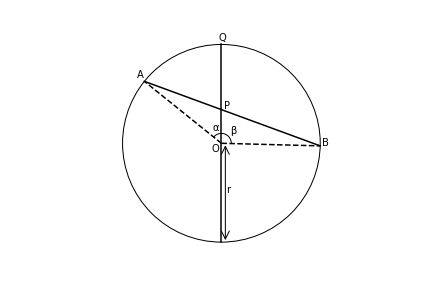
\includegraphics[width=\textwidth]{Diagram}

The areas of the top left and top right pieces can each be determined by subtracting the triangular area from the sector's area. Letting $\Delta_1$ and $\Delta_2$ be the top left and top right pieces' areas, respectively:
\begin{eqnarray}
\Delta_1 & = & \frac{1}{2}\alpha r^2 - |\triangle OAP| = \frac{1}{2}\alpha r^2 - \frac{1}{2}|\overline{OP}|r\sin\alpha \label{eq:Area1}\\
\Delta_2 & = & \frac{1}{2}\beta r^2 - |\triangle OBP| =\frac{1}{2}\beta r^2 - \frac{1}{2}|\overline{OP}|r\sin\beta \label{eq:Area2}
\end{eqnarray}
Also, points A and B are at $(-r\sin\alpha, r\cos\alpha)$ and $(r\sin\beta, r\cos\beta)$, respectively, so that the line connecting points A and B has the equation:
\begin{equation}
y = \frac{\cos\beta - \cos\alpha}{\sin\beta + \sin\alpha}x + \frac{\cos\alpha\sin\beta + \cos\beta\sin\alpha}{\sin\beta + \sin\alpha}r.
\end{equation}
It follows that:
\begin{equation}
\overline{OP} = \frac{\cos\alpha\sin\beta + \cos\beta\sin\alpha}{\sin\beta + \sin\alpha}r = \frac{\sin(\alpha + \beta)}{\sin\alpha + \sin\beta}r.
\end{equation}

Plugging this into Eqs.~(\ref{eq:Area1}) and (\ref{eq:Area2}) and solving for the values of $\alpha$ and $\beta$ that yield $\Delta_1 = \frac{1}{10}\pi r^2$ and $\Delta_2 = \frac{2}{10}\pi r^2$ gives
\begin{eqnarray*}
\alpha & = & 51.2\degree\\
\beta & = & 91.5\degree,
\end{eqnarray*}
which are the angles shown in the diagram.

\end{document}